% 2013_anhui_science_q15_fig1: schematic unit cube with P on BC and Q on CC1
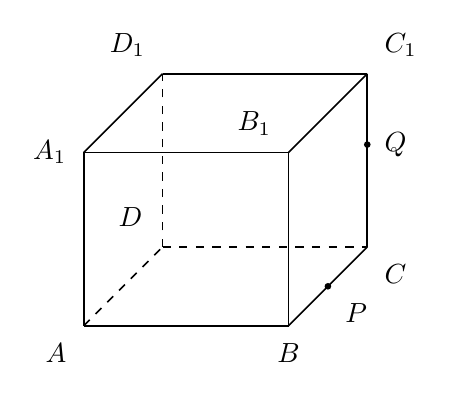
\begin{tikzpicture}[x=1cm,y=1cm,font=\normalsize,line width=.6pt]
\coordinate (A) at (0,0);
\coordinate (B) at (2.6,0);
\coordinate (B1) at (2.6,2.2);
\coordinate (A1) at (0,2.2);
\coordinate (D) at (1.0,1.0);
\coordinate (C) at (3.6,1.0);
\coordinate (C1) at (3.6,3.2);
\coordinate (D1) at (1.0,3.2);
\coordinate (P) at (3.1,0.5);
\coordinate (Q) at (3.6,2.3);
% front face
\draw[solid] (A) -- (B);
\draw[solid] (B) -- (B1);
\draw[solid] (B1) -- (A1);
\draw[solid] (A1) -- (A);
% top and right
\draw[solid] (D1) -- (C1);
\draw[solid] (C1) -- (C);
\draw[solid] (B) -- (C);
\draw[solid] (B1) -- (C1);
\draw[solid] (A1) -- (D1);
\draw[solid] (A) -- (A1);
% hidden
\draw[dashed] (A) -- (D);
\draw[dashed] (D) -- (C);
\draw[dashed] (D) -- (D1);
% points on edges
\fill (P) circle (1.2pt);
\fill (Q) circle (1.2pt);
% labels with clearance
\node[inner sep=2pt,below left=4pt] at (A) {$A$};
\node[inner sep=2pt,below=4pt] at (B) {$B$};
\node[inner sep=2pt,left=4pt] at (A1) {$A_{1}$};
\node[inner sep=2pt,above left=4pt] at (B1) {$B_{1}$};
\node[inner sep=2pt,above left=5pt] at (D) {$D$};
\node[inner sep=2pt,below right=4pt] at (C) {$C$};
\node[inner sep=2pt,above right=4pt] at (C1) {$C_{1}$};
\node[inner sep=2pt,above left=4pt] at (D1) {$D_{1}$};
\node[inner sep=2pt,below right=4pt] at (P) {$P$};
\node[inner sep=2pt,right=4pt] at (Q) {$Q$};
\end{tikzpicture}
